\documentclass[12pt]{article}
\usepackage{kotex}
\usepackage{graphicx}
\usepackage{amsmath}
\usepackage{hyperref}

\title{RetinaNet을 이용한 객체 검출 연구}
\author{Hochang Lee}
\date{\today}

\begin{document}

\maketitle

\begin{abstract}
객체 검출은 자율 주행, 감시 시스템, 로봇 공학 등 컴퓨터 비전 분야에서 중요한 연구 주제로, 최근 딥러닝 기술의 발전에 힘입어 검출 정확도가 크게 향상되었습니다. 본 연구에서는 텐서플로우와 KITTI 데이터셋을 활용하여 객체 검출 모델을 개발하고, RetinaNet 아키텍처의 성능을 분석하고자 합니다.
\end{abstract}

\section{Introduction}
RetinaNet은 ResNet-50을 backbone으로 하여 Feature Pyramid Network(FPN)를 결합한 구조로, 다양한 객체 크기에 대해 효과적으로 특징을 추출할 수 있습니다. 본 연구는 이러한 구조를 활용하여 자율 주행 환경에서의 객체 검출 성능을 높이는 것을 목표로 합니다.

\section{Model}
\begin{figure}[h!]
    \centering
    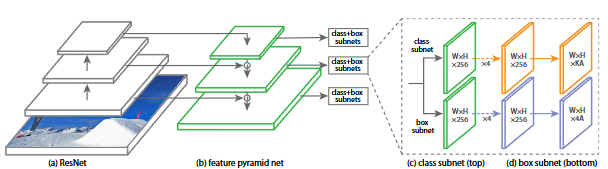
\includegraphics[width=0.75\linewidth]{image.png}
    \caption{RetianNet 모델 아키텍처}
    \label{fig:enter-label}
\end{figure}
RetinaNet 모델은 classification과 bounding box 예측을 위해 두 개의 서브네트워크(subnetwork)로 구성되어 있습니다. ResNet의 여러 층에서 추출된 feature map을 upsampling하여 결합하는 방식으로, 다양한 크기의 객체를 포착할 수 있습니다. 

\section{Loss}
학습에 사용된 loss 함수는 다음과 같습니다. Classification에 Focal Loss를 적용하였습니다. Focal Loss는 아래와 같이 정의됩니다. 
$$FL(p_t) = - (1 - p_t)^\gamma log(p_t)$$
여기서 $p_t$는 모델이 예측한 확률값을 나타내며, 정답 클래스일 경우 $p_t = p$, 정답이 아닌 경우 $p_t = 1 - p$로 설정됩니다. Bounding box 예측에는 Smooth L1 Loss를 사용하여 정확도를 높였습니다. 

\section{Data Set}
본 연구에는 자율 주행 연구에 널리 사용되는 KITTI 데이터셋을 사용하였습니다. 이 데이터셋에는 차량, 보행자, 자전거 등 다양한 객체에 대한 라벨이 포함되어 있습니다. 데이터셋은 학습, 검증, 테스트 세트로 나누어 사용하였으며, 학습된 모델을 실제 도로 이미지에 적용하여 객체 검출 성능을 평가하였습니다. 

\section{Experiments}
\begin{figure}[h!]
    \centering
    \begin{minipage}{0.45\linewidth}
        \centering
        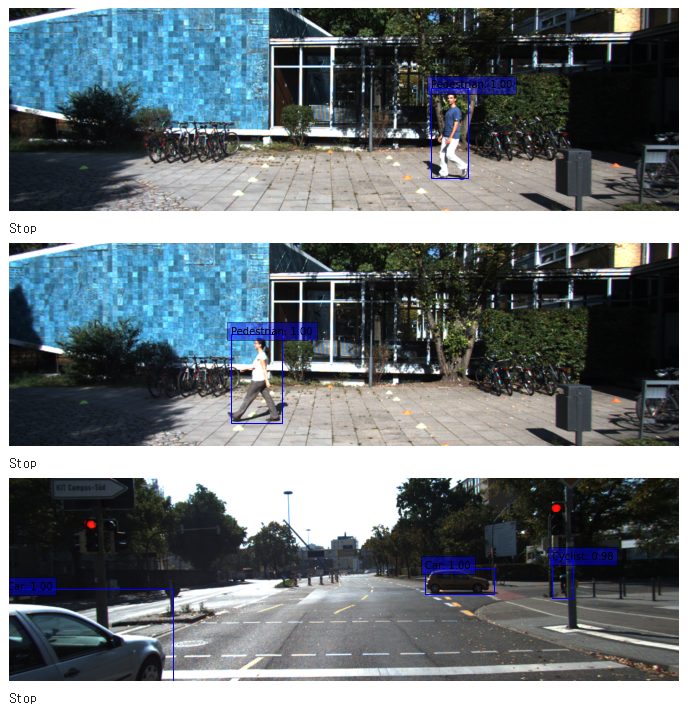
\includegraphics[width=\linewidth]{result1.png}
        \caption{모델이 이미지 내에서 근처의 보행자 혹은 가까이 있는 차를 탐지했을 경우, Stop을 출력하도록 합니다.}
        \label{fig:result1}
    \end{minipage}
    \hspace{0.05\linewidth} % 이미지 사이의 간격
    \begin{minipage}{0.45\linewidth}
        \centering
        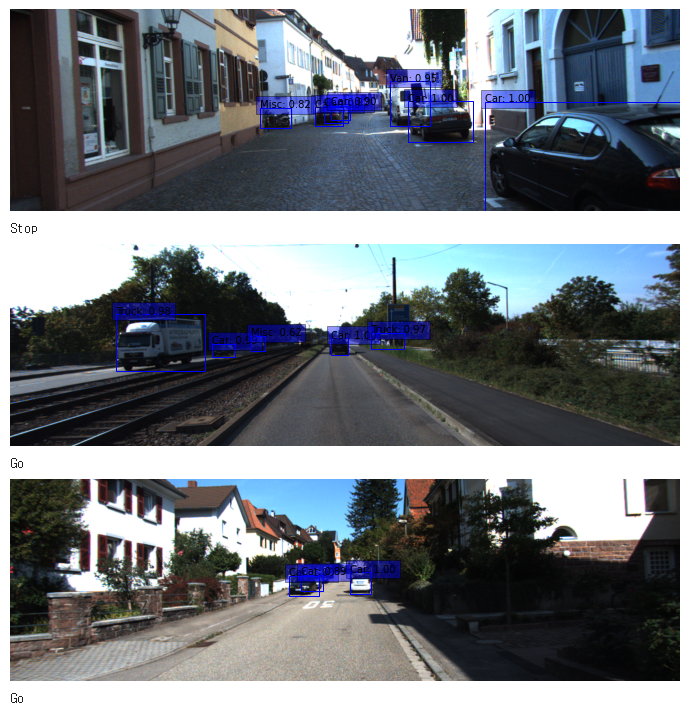
\includegraphics[width=\linewidth]{result2.png}
        \caption{모델이 이미지 내에서 근처의 보행자 혹은 가까이 있는 차를 탐지하지 않았을 경우, Go를 출력하도록 합니다.}
        \label{fig:result2}
    \end{minipage}
\end{figure}
본 연구에서는 제안된 RetinaNet 기반 객체 검출 모델이 실제 도로 환경에서 상황에 맞는 적절한 반응(Go 또는 Stop)을 출력할 수 있는지 평가하였습니다. 평가 과정에서는 다양한 상황을 나타내는 10장의 도로 이미지를 사용하였으며, 각 이미지에는 보행자 유무와 차량의 크기 정보를 포함하여 도로 상황을 반영하였습니다.

이미지 내에 보행자가 감지되거나 차량이 크게 검출되는 경우 \textbf{Stop} 신호를 출력하고, 그렇지 않은 경우 \textbf{Go} 신호를 출력하도록 설계하였습니다. 이와 같은 방식으로 모델이 실제 주행 환경에서 중요한 결정을 내릴 수 있는지 검토하였으며, 제안된 모델은 모든 테스트 이미지에 대해 정확한 예측을 수행하였습니다.

이 평가 결과는 제안된 모델이 도로 상황에서 실시간으로 객체를 인식하고 반응할 수 있는 가능성을 보여주며, 자율 주행 및 안전 운전 보조 시스템에 적용될 수 있음을 시사합니다.

\section{Conclusion}
RetinaNet을 활용한 본 연구는 자율 주행 환경에서 높은 객체 검출 성능을 확인하였으며, 다양한 크기의 객체에 대해 효과적인 특징 추출이 가능함을 보여주었습니다. 향후 연구에서는 더욱 다양한 환경과 객체에 대해 성능과 실시간으로 추론이 가능한지에 대한 성능도 검토할 예정입니다. 

\bibliographystyle{plain}
\bibliography{references}


\end{document}
